\documentclass[conference]{IEEEtran}
%\IEEEoverridecommandlockouts

\usepackage{cite, url}
\usepackage{amsmath,amssymb,amsfonts}
\usepackage{algorithmic}
\usepackage{graphicx}
\usepackage{textcomp}
\usepackage{soul} % for underlining
\usepackage{xcolor}
\pagecolor{white}
\usepackage{tabularx}
\usepackage{comment}
\usepackage{booktabs}

\def\BibTeX{{\rm B\kern-.05em{\sc i\kern-.025em b}\kern-.08em
    T\kern-.1667em\lower.7ex\hbox{E}\kern-.125emX}}
\begin{document}

\title{Short-Term Electric Load Forecasting in Smart Grids using Parallelisation and Hidden Markov Models}

\author{
\IEEEauthorblockN{Pulak Mehrotra and Sandeep Joshi
\IEEEauthorblockA{\textmd{Department of Electrical and Electronics Engineering}\\
{Birla Institute of Technology and Science Pilani, Rajasthan 333031, India}\\ 
E-mail: f20210017@pilani.bits-pilani.ac.in and sandeep85joshi@gmail.com}}}

\maketitle

\begin{abstract}
In this study, a new technique is proposed to model and predict short-term electrical load. Load forecasting is one of the most integral parts of power system planning and operation. The proposed technique aims to provide a better representation of a household's true power requirements by considering a household as a collection of appliances, with each device modeled using a separate Hidden Markov Model (HMM). The methodology also operates under the assumption that each appliance functions under a fixed number of states, each with its own unique power requirement, which is often misrepresented by the readings of the smart meter. To evaluate the performance of the proposed methodology, it is compared with various neural networks, which have become the industry standard. Detailed power usage information obtained from households (and the corresponding appliances) in Austria and Italy (GREEND) is used as benchmark data to evaluate the proposed algorithms. The proposed strategy outperforms similar neural network architectures in short-term load forecasting precision and accuracy.
\end{abstract}

\begin{IEEEkeywords}
Keywords. *please tell what to add here*
\end{IEEEkeywords}
\section{Introduction}

In order to supply electric energy to the customer in a secure and economical manner, an electric company faces many challenges in operation of the grid with the most prominent being power scheduling, load flow analysis, planning and control of the electric energy infrastructure. All of these problems could, in theory, be handled appropriately if the utility providers are aware of how the electric demands fluctuate with time. Load forecasting and modelling have been found to be one of the best-emerging fields of research to aid in solving such a problem. Load forecasting can be defined as a finding the difference between current and future load demand. Load forecasting minimizes utility risk by predicting future consumption of commodities transmitted or delivered by the utility. 

Load forecasting in smart grid-based power systems can be differentiated based on the time frame of the forecasts, namely short-term and long-term. Short-term load forecasting (STLF) has been found to be particularly helpful in smart grid functioning, as it allows the optimal scheduling of energy resources and the efficient management of energy storage systems. STLF relies on data modelling (fitting data to models, extrapolation, etc.) rather than on intimate information about how an electrical system works. Generally, STLF involves modelling power readings as time series models using historical data to identify patterns and trends in the load profile and make predictions based on the same.  

Broadly, load forecasting techniques can be divided into either parametric or non-parametric techniques. Parametric methods  involve building the load model putting an emphasis on the relationship between load and load-impacting factors, with the adequacy of the model being assessed based on the forecast errors as model residuals. Parametric methods mainly include statistical models, including but not limited to linear regression models, stochastic process models, exponential smoothing and ARIMA models \cite{regr1}. Non-parametric models handle nonlinear and non-monotonic relationships better than parametric models and automatically learn complex patterns and relationships in the data \cite{np1}-\cite{np2}. Hybrid models combine the strengths of multiple model classes, such as ANNs and time series models, to achieve better accuracy and robustness \cite{h1}-\cite{h2}.

With the advancements in machine learning technologies and the ease of their deployment at scale, one of the most popular and efficient methods of STLF has come out to be using artificially intelligent algorithms. One of the most common algorithms is the Artificial Neural Network (ANN) as done in \cite{generalnn3}, where imperative information regarding the movement patterns of the power readings is obtained based on the multiple time lags of chronological hourly peak load fed as input to the ANN. Some Convolutional Neural Network (CNN) based models have shown promising results, where the dimensions of the convolutions applied can be varied. In \cite{generalnn2} a 2D CNN based STLF model is proposed for the state of Goa in India. Fuzzy Logic (FL) could also be applied to the problem of short-term load forecasting in electrical power systems. To help in select the correct load-impacting factors from a dataset, feature selection is found to improve the performance and reduce the computation simultaneously as observed in \cite{fuzzy}. 

However, few challenges still need to be resolved with one of the largest being how the data is collected from a household. The smart meters used to transmit the power reading of a household or an appliance, often send wildly incorrect values owing to the erratic behaviour of the sensor involved. This leads to a dateset which often doesn't fully represent the reality of the needs of the connected load. Most of the existing forecasting approaches work without completely addressing this problem. Another existing problem is the fact that a single model increases chances of single point failure of the system as well as being more complex to work with.

To address these challenges, a stochastic model based on parallelisation is suggested in this paper. The major contributions of this paper are:
\begin{itemize}
    \item We propose a feature simplification framework that helps eliminate erroneous readings in smart meter readings, while still retaining the patterns in their data. That is, the proposed feature extraction framework transforms a time series, which consists of electrical load data and exogenous information, into a far more compact and simple form to facilitate STLF.
    \item Use of the proposed approach to efficiently determine the actual power fluctuations in microgrids, along with a comparative analysis between various techniques for load forecasting and feature extraction in smart grids. A general advantage of such a parallelised model over a monolithic model would be that it becomes clear which consists of connected device is responsible for the observed variation from the norm. 
    \item A deep learning-based approach is also proposed to forecast the load of smart grids accurately and with a reduced dependence on a single model, using the concept of load division and harnessing the power of stochastic models.
\end{itemize}

The paper is structured as follows. Section II introduces the various methodologies used in the paper's implementation, namely various versions of Recurrent Neural Networks and Hidden Markov Models (HMMs). The architecture used for forecasting in the paper is laid out in section III. Section IV discusses the details of the experiments on short-term load forecasting performed in this paper. Section V contains detailed evaluation results of the experiments performed. Finally, the conclusion and future work directions are placed in Section VI.

\section{Methodology}

\subsection{Recurrent Neural Networks (RNNs)}

An RNN is a neural network that works on the principle of a feedback loop, saving the output of a particular layer and feeding it back to the input to predict the output of that layer. Recurrent networks use their feedback connections to store representations of recently input events in the form of activations. This enables it to show dynamic behaviour that is only present for a short period, making it perfect for Time Series Forecasting.

\vspace{5pt} % Adjust the vertical space as needed

\begin{itemize}
    \item \textbf{LSTM} is a specialised type of RNNs that is specifically designed to capture the long-term dependencies in data, making them ideal fits for sequence prediction. Information can be reviewed and then appended or removed from the cell state using gates. These gates let the information flow in and out of the cell depending on the data's relative importance. 
\end{itemize}

\begin{itemize}
    \item \textbf{GRU} has two gates while the LSTM has three, which leads to LSTM performing more computation and training more slowly compared to GRU networks. The GRU does not possess any internal memory as it doesn’t have the output gate present in the LSTM. In GRU, the gates work directly with the previous hidden state.
\end{itemize}

\begin{itemize}
    \item \textbf{BiLSTM} is a type of sequence model which contains two concurrent LSTM layers, one for processing input in the forward direction and the other for processing the very same data in the backward direction.
\end{itemize}

\subsection{Hidden Markov Models (HMMs)}

HMMs are mathematical models which use hidden states to model observable data. The foundational principle of such models involves determining the \textit{hidden state sequence} corresponding to the observed data sequence and learning model parameters from the history of the observed data sequence. Hidden states are denoted by $s_t$.

The states are called "hidden" as we can not observe the states themselves but only the result of some probability function, known as an \textit{observation}, denoted by $o_t$. In a standard HMM, the states are in discrete form whereas the observations can either be discrete or continuous. Each state has a one-to-one mapping to an observation.

\begin{figure}[htbp]
  \centering
  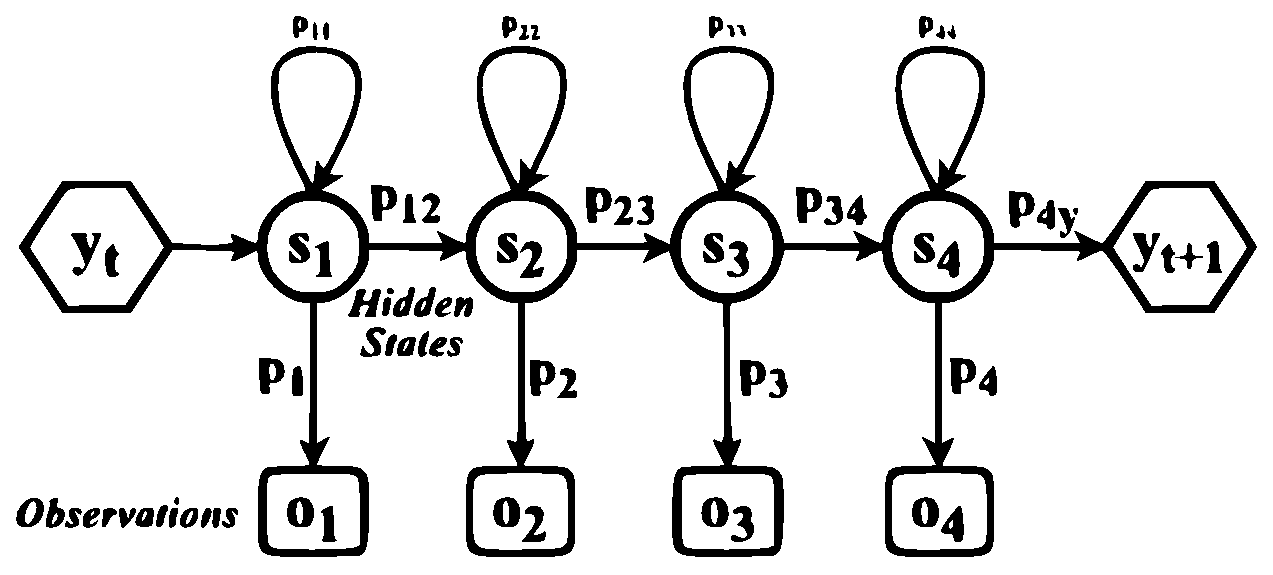
\includegraphics[width=0.4\textwidth]{HMM.eps}
  \caption{Topology of a HMM used for Prediction}
  \label{fig:hmm_exp}
\end{figure}

To achieve proper modelling of HMMs, apart from the set of hidden states and the set of output states, the Hidden Markov Model has three computable parameters:

\subsubsection{Transition Matrix ($A$)}

The State Transition Probability (A), which makes up the Transition Matrix, is the probability that a model from a hidden state  at time instant $t$ will make a transition to another hidden state at time instant $t$+1. Mathematically: 
\[ A_{ij} =  P(s_i | s_j \,)  \text{ where } i \text{ and } j \in \{1, 2, \ldots, N\}\]

\subsubsection{Prior Probability ($\pi$)}
Helps determine which state the model will start from, out of the states available in the set of hidden states. Mathematically:
\[
\pi_i = P(x_1 = i) \text{ where } i \in \{1, 2, \ldots, N\}
\]

\subsubsection{Emission Probability ($B$)}
Helps determine which observation a state will lead to. Mathematically:
\[ B = P(o_t | s_t)\]

Forecasting using HMMs aims to predict the most likely observational output sequence for a given model, using the computed hidden state sequence based on historical data. Finding which observation corresponds to a given hidden state is commonly known as \textit{decoding}. This problem can be solved using the \textit{Viterbi algorithm}, which works under the assumption that in an HMM the next state only depends on the previous one. The principle of the Viterbi algorithm involves recursively simplifying a complicated problem by breaking it down into simpler sub-problems. It computes the probability of the most likely path up to each state at each time step using and is computed using a dynamic programming map called a \textit{trellis}, as shown in Fig. 4.

\begin{figure}[htbp]
  \centering
  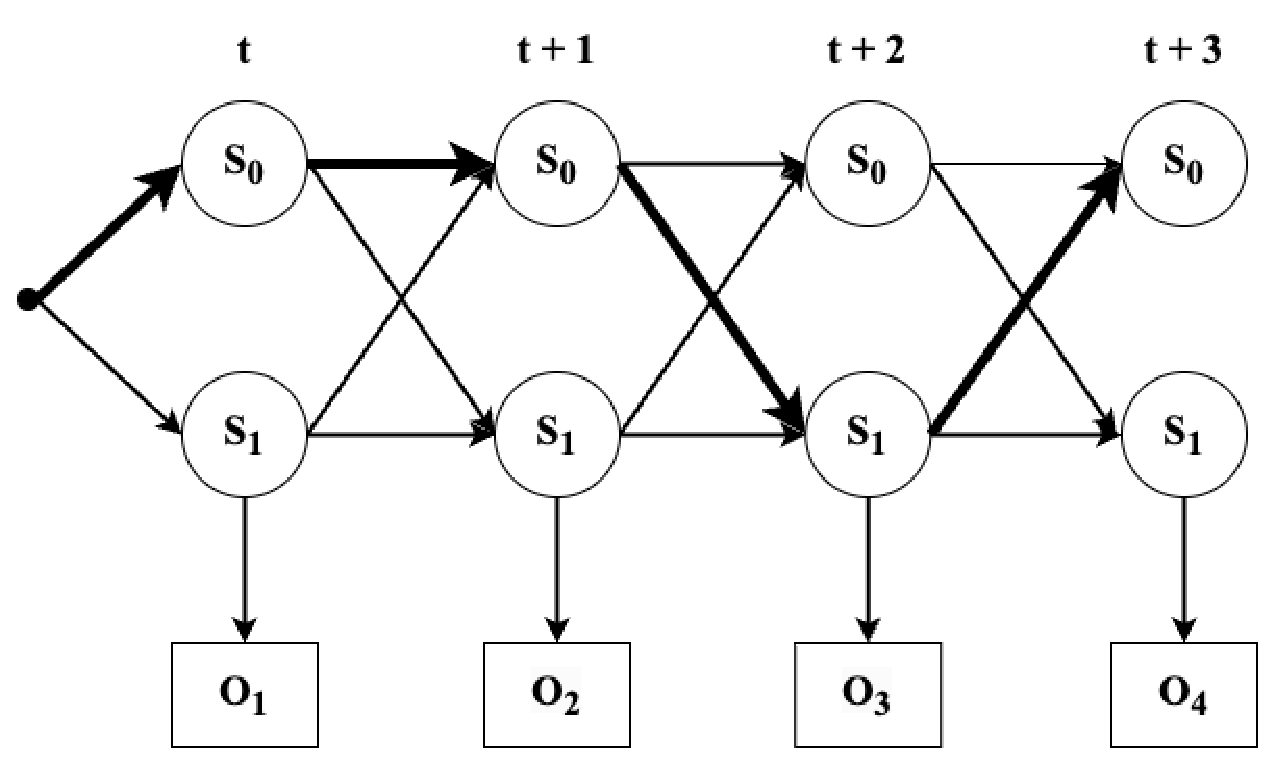
\includegraphics[width=0.4\textwidth]{Trellis.eps}
  \caption{Simple Two-State Trellis using Viterbi Decoding.}
  \label{fig:trellis}
\end{figure}

\section{Proposed Models}
In this section, we present the design considerations and architecture of our short-term electric load forecasting system.
\\
\textcolor{red}{should i add any assumptions here?}

\begin{figure}[htbp]
  \centering
  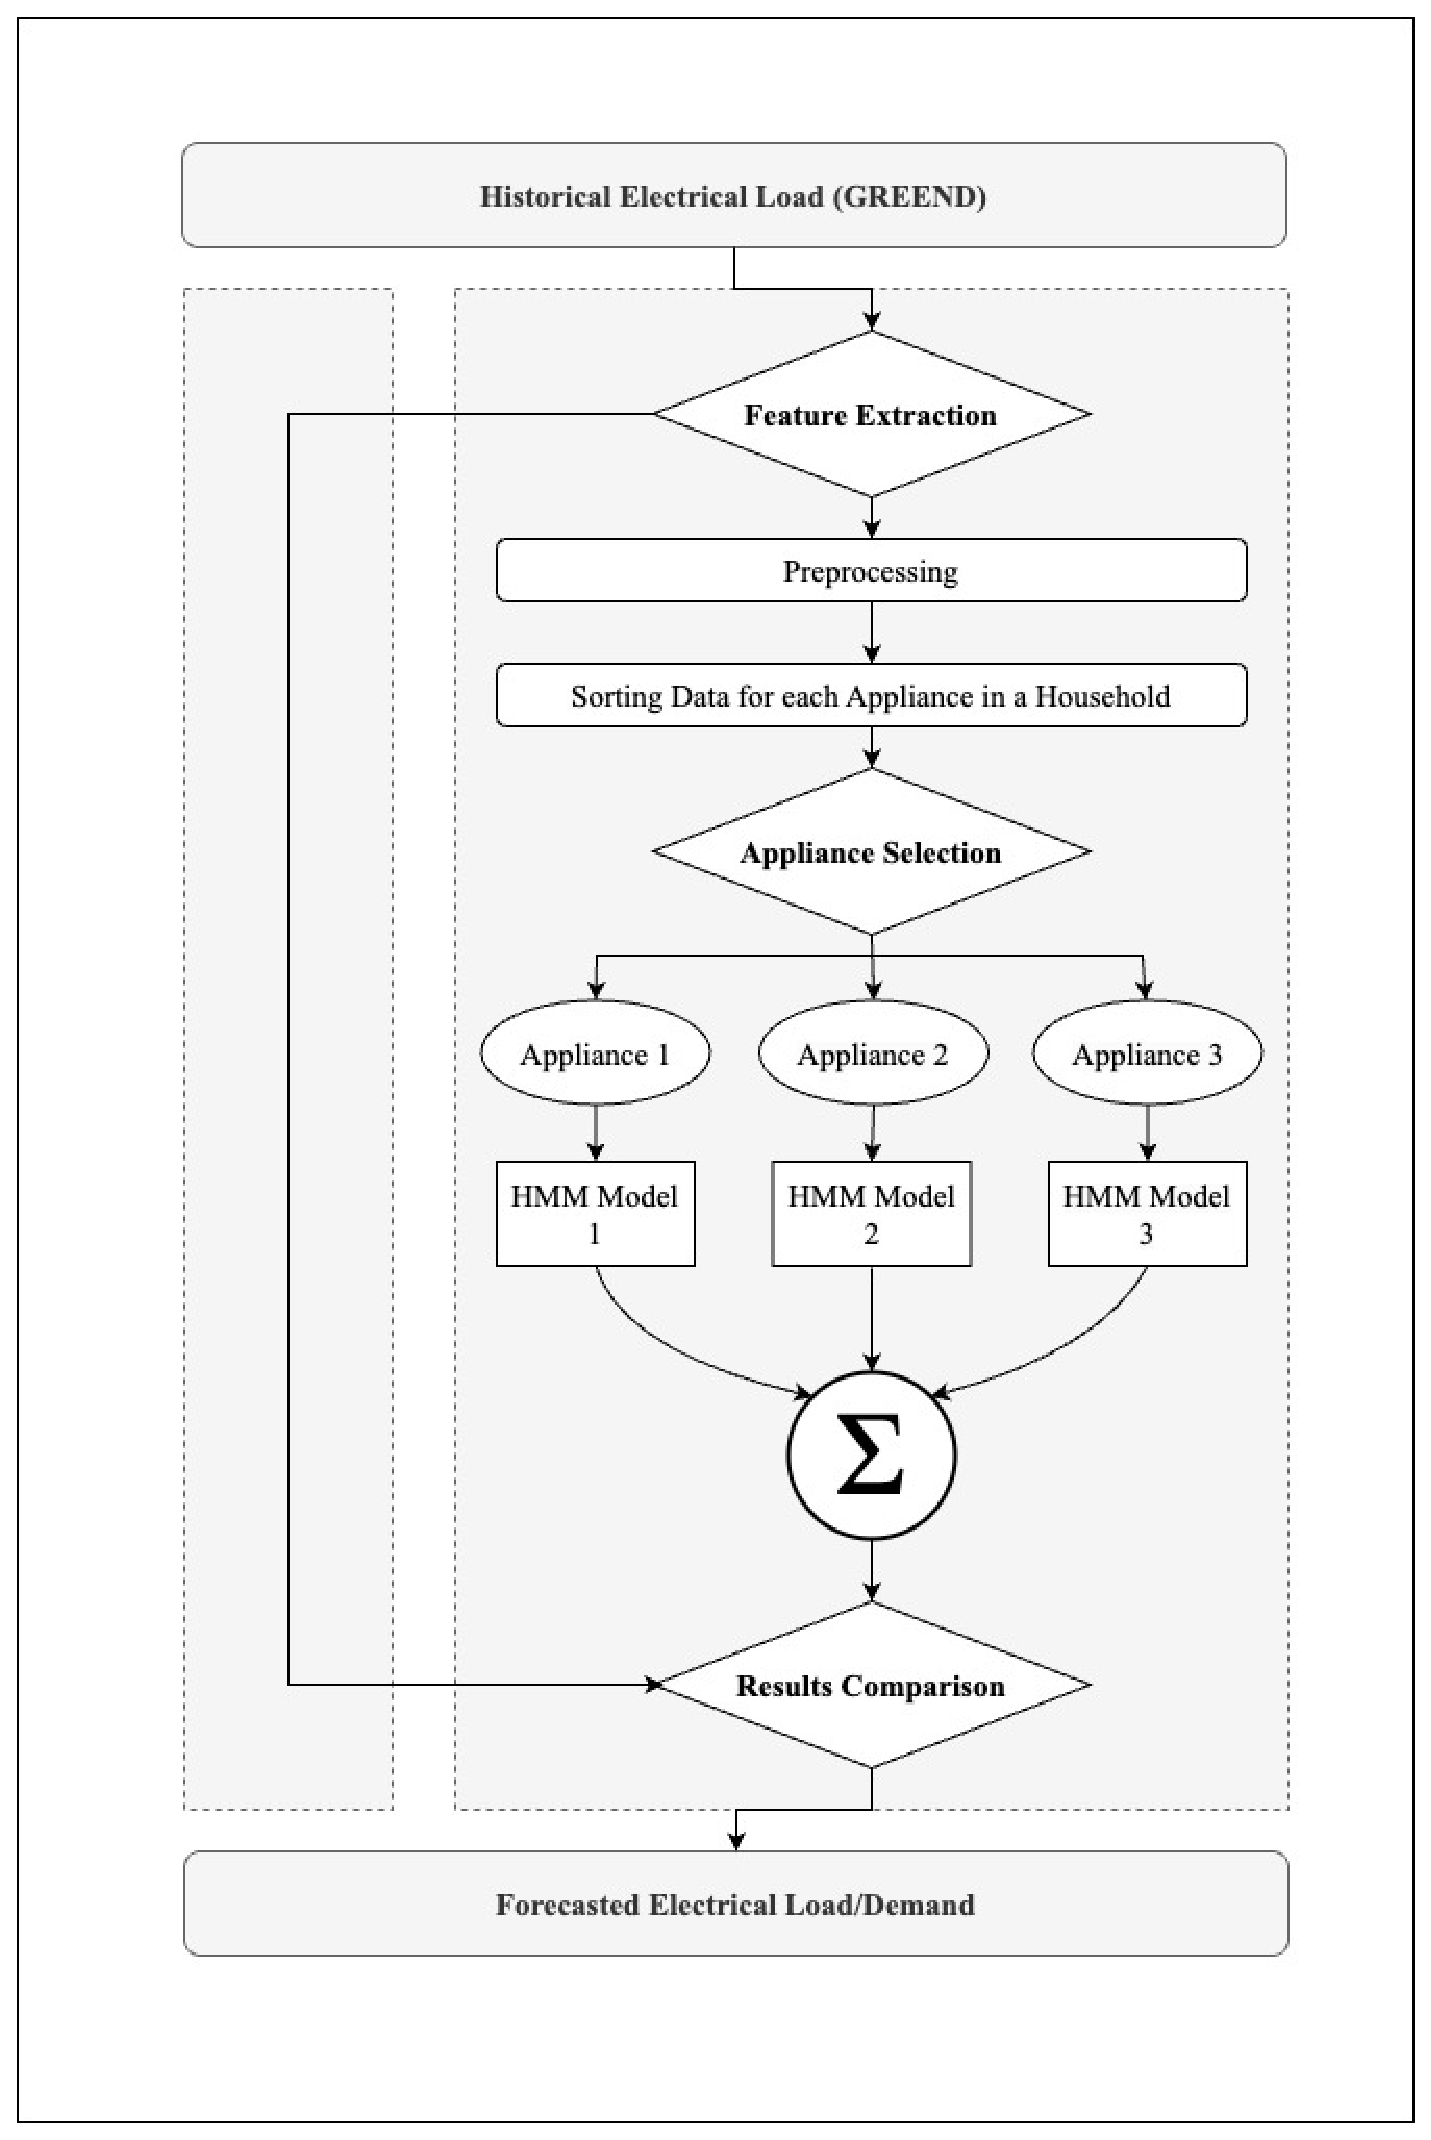
\includegraphics[width=0.4\textwidth]{HMM_Model.eps}
  \caption{Proposed Neural Network Forecasting Model.}
  \label{fig:hmm_model}
\end{figure}


\begin{figure}[htbp]
  \centering
  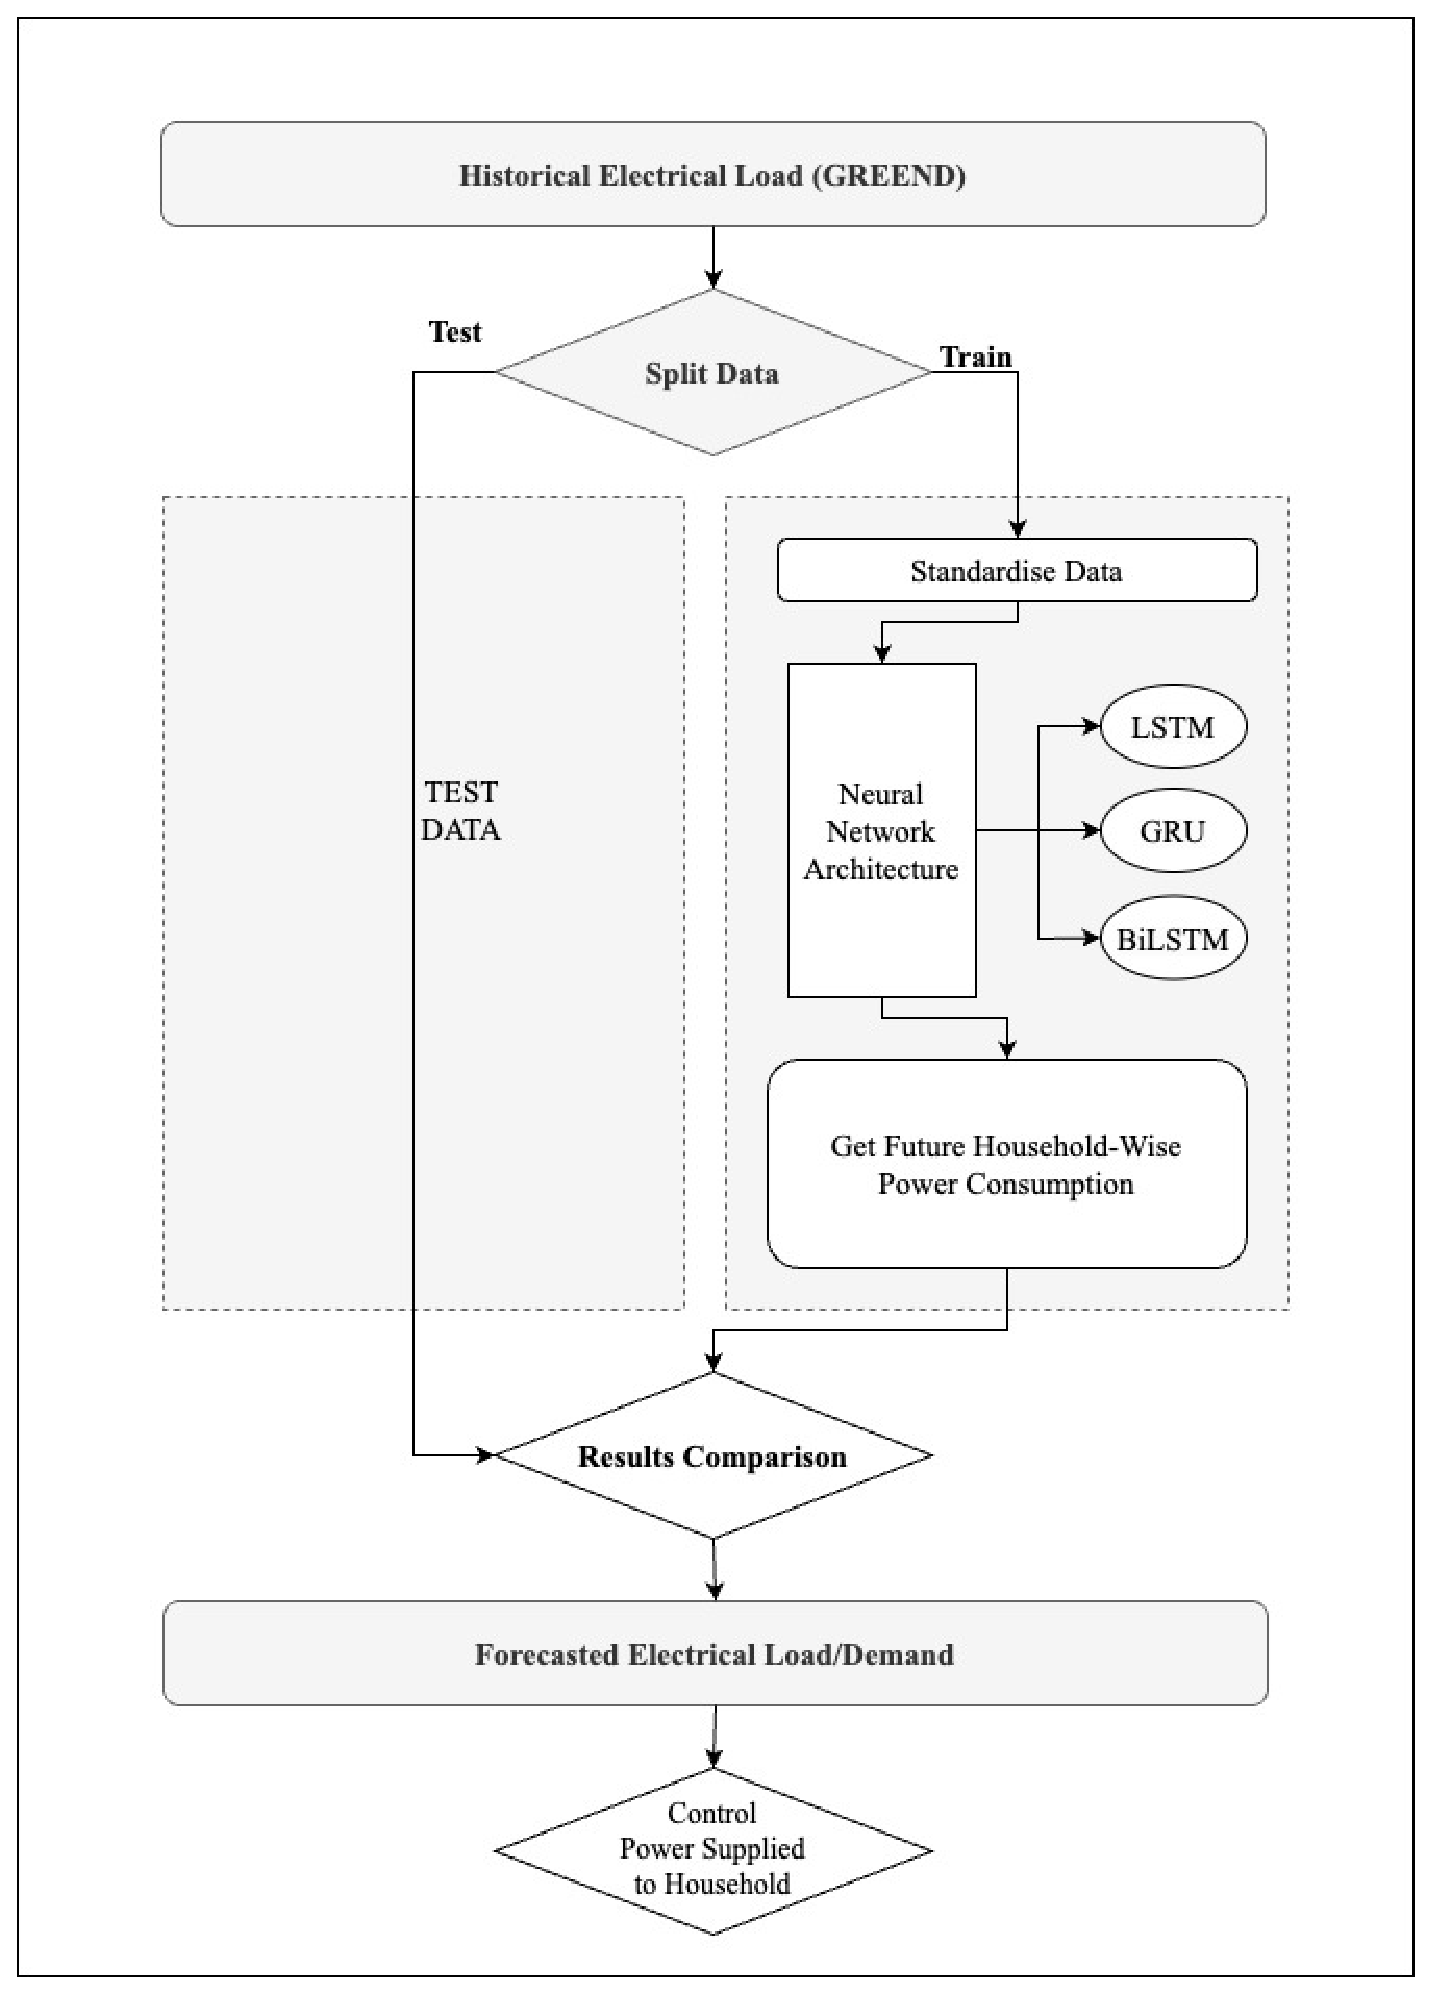
\includegraphics[width=0.4\textwidth]{NN_Model.eps}
  \caption{Proposed HMM Forecasting Model.}
  \label{fig:nn_model}
\end{figure}

The electricity load demand data set used in this paper is the GREEND \cite{greend} dataset, which contains the detailed power usage information obtained through a measurement campaign in households in Austria. The household and appliance wise data is used to train the prediction models and verify the authenticity of the proposed model performance and while the data set covers the load behaviour for over two years, we used a smaller timeframe to test the proof of the concept of our proposed model. Similarly, we only used the data from three appliances (radio, dishwasher and lamp) from a single building (Building 1) in the GREEND dataset to simplify computation for the models proposed in this paper. 

\subsection{Proposed Neural Network Forecasting Model}
The industry usually uses neural networks to model loads for households \cite{generalnn1}- \cite{generalnn4}. We've used a generalised approach, consisting of parts of each of the mentioned papers. In the preprocessing step of this approach, the reduced dataset is split into two parts: Test and Train. Further preprocessing involves standardizing all the involved data to the Train portion of the dataset. Following the preprocessing, the Train data is then fed as into the neural network model to enable the models to recognize and learn the patterns in the historical data.

Household wise data is first normalised and then fed as input to the Neural Network model used for forecasting. The neural networks used in the model are each composed of two layers, with the output of these layers passed through the activation function layer. 

\subsection{Proposed HMM Forecasting Model}
One fundamental idea in engineering involves the conversion of problems from a complex or less manageable form to a simpler, more informative form. Parallelisation of processes allows many calculations or processes are carried out simultaneously. This very idea is applied here in this model. As shown in Figure 4, three separate HMMs are used in the model, namely, HMM1, HMM2 and HMM3, with each HMM modelling the power readings for a particular appliance. However, before feeding data into the HMM we performed we have to perform \textbf{state selection} of the input data. 

A household consists of many appliances, which have been assumed to each individually consume a certain amount of power at a given instant, totalling to the overall power demand of a household at a given instant. Now, logically, each appliance has a fixed number of states (using the definition mentioned above) it functions in, with each state having a certain fixed power requirement. For example, assume a Washing Machine could has five states : 'OFF', 'HIGH POWER WASH', 'LOW POWER WASH' and 'DRY'. Each state if the appliance will have a fixed power usage, and even accounting for power fluctuations in the devices, that should lead to not more than 3-4 readings per state. Instead, on observing the GREEND dataset, it was found that each appliance had over 50 unique power readings, some with as little as one occurrence. 

To remove the majority of the erroneous readings, we assumed each appliance had a fixed number of state and a single reading per state, with the readings being the ones with the highest occurrence. This greatly simplifies the data sequence, while maintaining the overall trend of the data sequence. This simplified data is fed as input to the HMMs and the predictions from each appliance's HMM are individually summed to give the prediction for the household in general.

\section{Experiments and Results}
The system comprises several key components that work together to achieve accurate load forecasting. This section provides an overview of these components and their interactions. Here the values are predicted by implementing the machine learning models using the Keras Library in the TensorFlow framework, while the HMM-based prediction is implemented using the hmmlearn Library in Python. 

\subsection{Evaluation Indices}

In this paper, Mean Absolute Percentage Error (MAPE), Mean Absolute Error (MAE) and Mean Absolute Error (MAE)are used as evaluation indices [8] to evaluate the prediction level of the model. These indices are calculated as in (1), (2) and (3) where $n$ is the number of data points, $y_i$ is the actual value, and $\hat{y}_i$ is the predicted value. MAPE is specifically used in this paper to compare models which have the input data in different form. 

\begin{equation}
\text{MSE} = \frac{1}{n} \sum_{i=1}^{n} (y_i - \hat{y}_i)^2
\end{equation}

\begin{equation}
\text{MAE} = \frac{1}{n} \sum_{i=1}^{n} |y_i - \hat{y}_i|
\end{equation}

\begin{equation}
\text{MAPE} = \frac{1}{n} \sum_{i=1}^{n} \left(\frac{|y_i - \hat{y}_i|}{|y_i|}\right) \times 100
\end{equation}

\subsection{Data Collection and Pre-Processing}

The LSTM NN based forecasting models are benchmarked by using an LSTM layer with 64 units followed by two dense layers with ReLU and linear activation functions, respectively. The single step ahead model is implemented with a 10-step look-back window. The BiLSTM NN model also consists of two stacked Bidirectional LSTM layers. The first layer returns sequences  to provide temporal context to the subsequent layer. A Dense layer with one unit is added as the output layer to predict the next value in the time series. The GRU NN consists of two GRU layers with dropout regularization to prevent overfitting, followed by a dense output layer.

\begin{table*}[htbp]
\centering
\caption{Performance Metrics for Different Neural Network Models}
\begin{tabular}{lccc}
\toprule
Model Name & Loss & MSE & MAPE \\
\midrule
LSTM      & 0.015797    & 0.000367    & 0.007271 \\
GRU       & 0.134251    & 0.021198    & 0.047211 \\
BiLSTM    & 0.014626    & 0.000321    & 0.011920 \\
HMM Model & 0.07025     & 0.035125    & 0.035125 \\
\bottomrule
\end{tabular}
\end{table*}

*cite tables*

Table [xxx] presents the results of various forecasting models on dataset 1 when the machine learning models used are LR, LSTM, and DNNs. When accuracy is considered, the best-performing model is the LSTM model, but what is to notw is that the GRU outperforms the GRU model and is fairly close to the .*

\begin{figure}[htbp]
  \centering
  \includegraphics[width=0.5\textwidth]{NNvsActual.eps}
  \caption{Comparison of the Forecasted and Actual Load for the Neural Network-Based Models.}
  \label{fig:nn_vs_a}
\end{figure}

The comparison of a parallelization-based STLF model using Hidden Markov Models is illustrated in Fig. *xxx*. The independent axis represents the time points and the dependent axis represents the energy consumption in kWh. The results in the figure denote that the proposed methodology has generated accurate predictions, and that this model predicts energy consumption values close to it better than the actual values of consumption for all machine learning algorithms in general. 
*expand which chosen method is the best*

\begin{figure}[htbp]
  \centering
  \includegraphics[width=0.4\textwidth, height=0.35\textwidth]{HMMvsActual.eps}
  \caption{Comparison of the Forecasted and Actual Load for the HMM Model.}
  \label{fig:hmm_vs_a}
\end{figure}

figure{nnvsa} - shows how the neural network models' predictions differ from that of the actual load. figure{hmmvsa} does the same but for the hmm model. losses are mentioned in figure{losses} 

\begin{figure}[htbp]
  \centering
  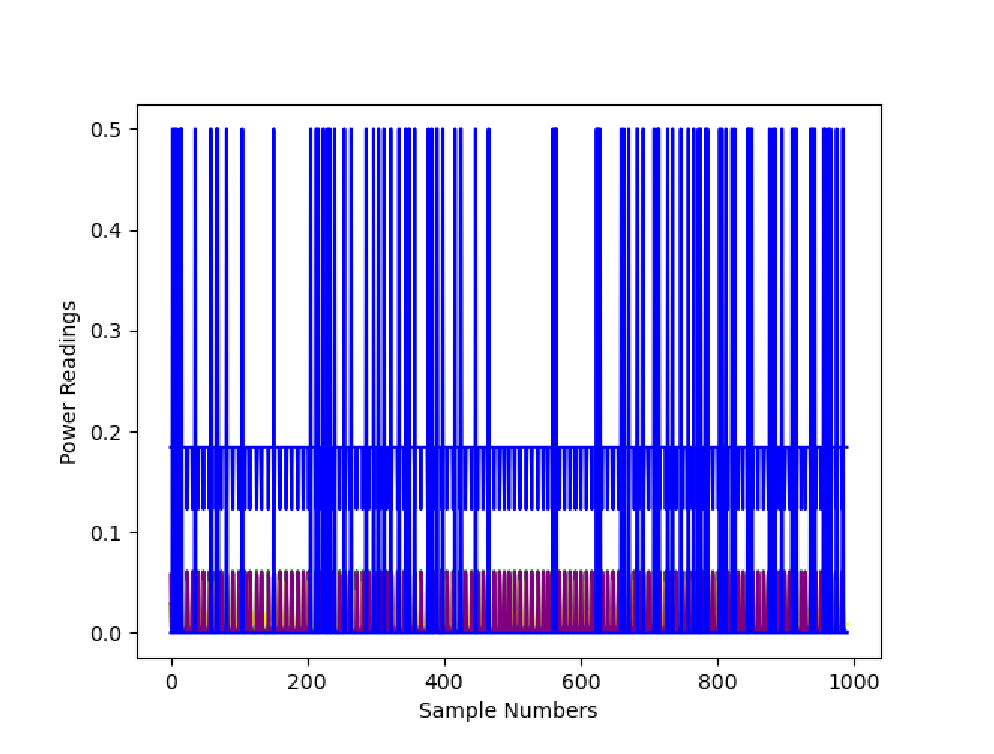
\includegraphics[width=0.5\textwidth]{losses.eps}
  \caption{Comparison of the Losses between the Actual and Predicted Load for the HMM Model and the NN Models.}
  \label{fig:loss}
\end{figure}

\begin{comment}
As found in the experiments, the results obtained by ELM and H-ELM varied greatly with each run. Therefore 1,000 runs were repeated for both algorithms. The results are listed in Table 3, in which H-ELM outperform ELM significantly. 

Figure 3 compares the  post-sample forecasting accuracyof the three Holt–Winters methods and the ARIMA modelfor lead times up to a day-ahead. The figure shows the meanabsolute percentage error (MAPE) ,which is the most widelyused error summary measure in electricity demand forecast-ing.  Following  the  recommendation  of  Hippertet  al,9wealso  calculated  the  mean  absolute error ,root-mean-squareerror ,and root-mean-square percentage error ,but we do notreport these results here because the relative performances ofthe methods for these measures were very similar to those forthe  MAPE.  The  results  for  Holt–Winters  for  within-dayseasonality were so poor that it was impractical to plot theMAPE values beyond 2 steps ahead on the same graph asthe MAPE values for the other methods. This is due to themethod  failing  to  accommodate  within-week  seasonality.This  might  have  been  anticipated  from  Figure  1  ,whichshows  how  very  different  the  demand  on  Saturdays  andSundays is from that on weekdays. Holt–Winters for within-week seasonality is far more competitive ,suggesting that thewithin-week seasonality accounts for a large proportion ofthe variation in the data. However ,double seasonal Holt–Winters outperforms Holt–Winters for within-week season-ality  for  38  of  the  48  lead  times  ,indicating  that  there  isbenefit  in  using  a  method  that  is  able  to  pick  up  bothseasonalities. Beyond 12 hours ahead ,the accuracy of thesetwo methods tends to improve with the lead time. This is due to the within-day seasonality ,and it implies that a forecastfor 12 h ahead would be better made from a forecast origin12 h  prior  to  the  current  period.  In  his  analysis  of  onlinemethods ,Smith18also concludes that the choice of forecastorigin  should  depend  on  the  forecast  horizon.  Comparingthe  two  double  seasonal  methods  ,we  see  that  doubleseasonal   ARIMA   outperforms   double   seasonal   Holt–Winters for all but the last 5 lead times

igure 4 shows the post-sample forecasting performancefor  the  three  Holt–Winters  methods  with  residual  auto-correlation   adjustment.   The   MAPE   results   for   doubleseasonal ARIMA ,which were plotted in Figure 3 ,are alsoshown  in  Figure  4.  The  new  results  for  all  three  Holt–Winters methods have improved substantially from Figure 3.The  relative  performance  of  the  three  methods  has  notchanged ,but double seasonal Holt–Winters is now the bestof the three for all 48 lead times. Interestingly ,the methodnow also outperforms double seasonal ARIMA for all thelead times. Beyond 12-periods ahead ,the ARIMA model isalso outperformed by Holt–Winters for within-week season-ality
\end{comment}

\section{Conclusions}

Two intelligent forecasting approaches were proposed and evaluated in this paper. The performance and applicability of these solutions were compared with each other, with one method being the general approach to STLF in the industry and the second being a improved version of the same. Feature/State extraction is used to reduce dimensionality and redundancy in order to give more relevant input to the HMM Predictor. It is shown that the proposed HMM based model can produce a prediction accuracy comparable to that of a RNN model, in fact performing better than the GRU and decently comparable to that of the LSTM-based models. In essence, the parallelised models were found to be highly competent compared to the machine learning models in terms of accuracy of short term predictions.

During the prediction two or more models can be used for same dataset, to find the accuracy of each model and also find which model is appropriate for predicting the load demands. Additionally, the number of states on which this prediction is based, can also be varied depending on the specific use case of the implementation. Along with this, future work could include further improving the methods of state assumption, while using as few assumptions as possible. The proposed methodology can be used with huge electrical networks and big data in smart grids at any level. Future work will investigate the scalability of the proposed methodology to a large electrical distribution network, as well as other methods of state selection to simplify the data sequences.

\bibliographystyle{IEEETran}
\bibliography{main} % without the .bib extension
\vspace{12pt}
\end{document}
